\documentclass[oneside,13pt,a4paper]{report}

% Chargement d'extensions
\usepackage[utf8]{inputenc}
\usepackage[french]{babel}
\usepackage{graphicx}
\usepackage[top=3cm, bottom=3cm, left=3cm, right=3cm]{geometry}

\usepackage{amsmath}
\usepackage{amssymb}

% csquotes va utiliser la langue définie dans babel
\usepackage[babel=true]{csquotes}
 
% pour afficher Schéma au lieu de figure dans les legende des images
\addto\captionsfrench{\def\figurename{Schéma}}

% Informations le titre, le(s) auteur(s), la date
\title{Moteur de Requêtes SQL Simples}
\author{
    Massili KEZZOUL \and
    Chakib ELHOUITI \and
    Ramzi ZEROUAL \and
    Belkassim BOUZIDI \and
    Fei YANG
}
\date{\today}


\begin{document}
%\maketitle
\begin{titlepage}
	\centering
	{\scshape\LARGE Univérsité de Montpellier\par}
	{\scshape\Large Rapport de projet\par}
	\vspace{1.5cm}
	{\huge\bfseries Moteur de requêtes SQL simples\par}
	\vspace{2cm}
	{\Large\itshape
		Massili KEZZOUL \\
		Chakib ELHOUITI \\
		Ramzi ZEROUAL \\
		Belkassim BOUZIDI \\
		Fei YANG \\
		\par}

	\vspace{1.5cm}

	{\Large\itshape
		Encadrante :\par
		Mme. Anne-Muriel \textsc{Chifolleau}
		\par}

	\vspace{2cm}

	\begin{figure}[h]
		\begin{minipage}[c]{.46\linewidth}
			\centering
			
\includegraphics[width=1\textwidth]{img/univ-montpellier.png}
		\end{minipage}
		\hfill%
		\begin{minipage}[c]{.46\linewidth}
			\centering
			
\includegraphics[width=1\textwidth]{img/fds.png}
		\end{minipage}
	\end{figure}

	\par\vspace{1cm}

	\vfill

	% Bottom of the page
	{\large \today\par}
\end{titlepage}




% ------------------------------------- %
% Introduction
% ------------------------------------- %

\parskip=5pt
\chapter*{Introduction}

Dans le cadre de notre second semestre de la Licence 2,
il nous est proposé un projet nous permettant de mettre en pratique nos connaissances et nos compétences
au travers d’un cahier des charges ayant pour finalité la conception et le développement d’un moteur d’évaluation de requêtes SQL en mémoire vive.

Les requêtes considérées seront des requêtes simples de la forme : \enquote{SELECT ... FROM ... WHERE ... }  sans imbrication.

À partir d’un ou plusieurs fichiers CSV, Comma-separated Values\footnote{Comma-separated values, format texte ouvert représentant des données tabulaires sous forme de valeurs séparées par des virgules. Voir page \pageref{csv}},
il est demandé de construire une représentation en mémoire des données et d’implémenter les procédures de projection,
sélection et de jointure découlant de l’interrogation SQL.

Il s’agit principalement de reproduire les fonctionnalités de bases d’un SGBD\footnote{Système de Gestion de Base de Données, voir page \pageref{sgbd}}, tel que MySQL ou bien Oracle.

Notre groupe, composé de cinq personnes : Massili Kezzoul, Chakib Elhouiti, Ramzi Zeroual, Belkassim Bouzidi et Yang Feï, et encadré par Mme Anne-Muriel Chifolleau,
a saisie l'opportunité de réaliser ce projet.

\chapter*{Remerciments}

\parskip=0pt
\tableofcontents

% Espacement entre les paragraphes
\parskip=5pt
% ------------------------------------- %
% Organisation
% ------------------------------------- %

\chapter{Organisation du projet}
\section{Méthodes d’organisation}

Afin de mener à bien le développement du projet, nous avons décidé de travailler un maximum de temps ensemble et de manière très régulière. Nous nous sommes réunis trois à quatre fois par semaine afin de faire le point sur l’avancement du projet et de définir les objectifs restant à atteindre.

Enfin, selon l’état d’avancement du moteur de requêtes, nous réalisons les tâches en retard durant le week-end pour ne pas cumulé de retard et respecter l’intégralité du cahier des charges.

Toutes les semaines, nous nous sommes réunis avec notre encadrante, Mme Anne-Muriel Chifolleau, afin de faire le point sur l’état du projet. Ces réunions nous on également permis de bénéficier des précieux conseils de notre encadrante.

\section{Decoupage du projet}

Nous avons découpé la réalisation du projet en trois grandes phases.

\subsection{Phase de modélisation}

Durant cette étape, nous nous somme réunis pour définir les fonctionnalités demandés par le projet. Notamment séparer les fonctionnalités importants de celle moins importantes. Nous avons également choisi les outils de travail collaboratif et les principales technologies utilisés, ainsi que une première modélisation du projet.

\subsection{Phase de développement}

Durant cette phase, nous avons commencer à implémenter les différentes fonctionnalités que nous avons modélisé lors de l’étape précédente, toute en améliorant la modélisation au fur et à mesure de l’avancement de notre projet. Nous avons notamment réaliser des tests pour les différents modules afin de s’assurer de leur bon fonctionnement.

\subsection{Finalisation du projet}

Cette étape a consisté en la réalisation des tests finaux afin de s’assurer que le moteur de requêtes fonctionne en toute circonstance et éventuellement corriger les bogues qui peuvent apparaître.

\section{Outils de collaboration}

Afin de s’organiser, nous avons décider d’utiliser Git au travers du serveur GitLab héberger par le service informatique de la faculté. En effet le logiciel libre Git a facilité grandement la collaboration entre nous. Le serveur GitLab quant à lui est fourni gratuitement par le service informatique la faculté.

% ------------------------------------- %
% Le langage SQL
% ------------------------------------- %

\chapter{Le langage SQL et les bases de données}

%Le domaine dans le quelle ce situ notre projet est la gestion d’une base de donnée en utilisant le langage SQL .

%\section{Qu’est-ce qu’une donnée}
\section{Présentation d’une base de donnée}

Une base de données regroupe et stock un ensemble d’informations, qu'on appelle aussi donnée.
En termes simples, les données peuvent êtres des faits liés à tout objet considéré.
(Par exemple, un nom, un age, une taille, un poids ...)

On s'interesse ici uniquement au base de données dite relationnelles, une base de données où l'information est organisée dans des tableaux à deux dimensions appelés des relations ou tables\footnote{ selon le modèle introduit par Edgar F. Codd en 1970.}.
Selon ce modèle relationnel, une base de données consiste en une ou plusieurs relations. Les lignes de ces relations sont appelées des nuplets ou enregistrements. Les colonnes sont appelées des attributs.

\begin{figure}[h]
	\centering
	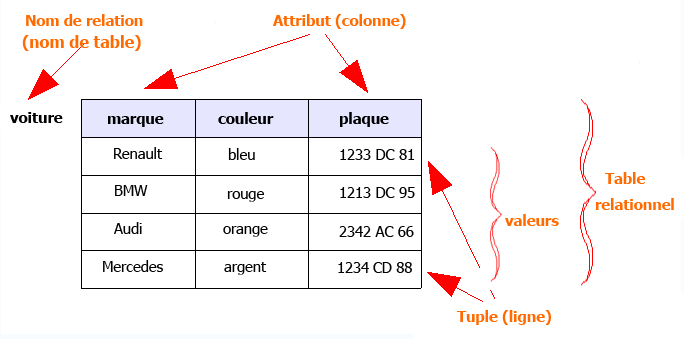
\includegraphics[width=0.7\textwidth]{img/table_relationnel.png}
	\caption{Représentation d'une Table}
\end{figure}

En informatique, une base de données est la pièce centrale des dispositifs de collecte, mise en forme, stockage et utilisation d'informations.
Ce dispositif comporte un système de gestion de base de données.

\section{Système de gestion de base de données}
\label{sgbd}
Le système de gestion de base de données (SGBD) est un ensemble de programmes qui permet à ses utilisateurs d'accéder à une base de données,
de manipuler des données, ainsi que de contrôler l'accès à la base de données, tout en cachant la complexité des opérations effectuer.

Les SGBD sont utilisés pour de nombreuses applications informatiques, notamment :
\begin{itemize}
	\item les guichets automatiques bancaires
	\item les bibliothèques numérique
	\item les logiciels d'inventaire
	\item et aussi dans de nombreux blogs et sites web.
\end{itemize}

%\vfill

\begin{figure}[h]
	\centering
	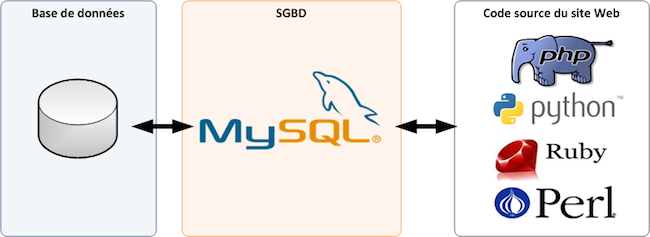
\includegraphics[width=0.7\textwidth]{img/sgbd.png}
	\caption{Représentation d'un SGBD}
\end{figure}

Il existe de nombreux SGBD. En 2008, Oracle détenait près de la moitié du marché avec MySQL et Oracle Database.
Les opérations de recherche et de manipulation des données peuvent être exprimées sous forme de requêtes (anglais query)
dans un langage informatique reconnu par le SGBD. SQL est le langage informatique le plus populaire.

\section{Le langage SQL}
\label{sql}

Le SQL (sigle de Structured Query Language, en français langage de requête structurée) est le langage standard pour traiter les bases de données relationnelles.
La programmation SQL peut être utilisée efficacement pour insérer, rechercher, mettre à jour et supprimer des enregistrements de base de données.
Les instructions SQL s'écrivent d'une manière qui ressemble à celle de phrases ordinaires en anglais. Cette ressemblance voulue vise à faciliter l'apprentissage et la lecture.

Le SQL est un langage déclaratif, c'est-à-dire qu'il permet de décrire le résultat escompté, sans décrire la manière de l'obtenir.
Les SGBD sont équipés d'optimiseurs de requêtes, des mécanismes qui déterminent automatiquement la manière optimale d'effectuer les opérations,
notamment par une estimation de la complexité algorithmique.

Le langage SQL est utilisé par des bases de données relationnelles, telles que la base de données MySQL, Oracle, le serveur Ms SQL, Sybase, etc...

Les instructions SQL couvrent 3 principale domaines :
\begin{itemize}
	\item langage de manipulation de données.
	\item langage de définition de données.
	\item langage de contrôle des données et des transactions.
\end{itemize}
\vspace{0.3cm}

Le domaine considéré dans ce projet et le langage de manipulation de données simple sans imbrication.
Example de requête SQL : \enquote{SELECT Name FROM Members WHERE Age $ \leq $ 30;}

% -------------------------------------------------------------------------- %
% Présentation du projet : moteur de requêtes SQL simples
% -------------------------------------------------------------------------- %

\chapter{Présentation du projet : moteur de requêtes SQL simples}

\section{Présentation générale}

Notre projet consiste à concevoir et implémenter un programme capable de lire des données, executer des requêtes SQL simple en mémoire et de renvoyer le resultat.
Il s’agit donc de crée une passerelle entre la personne qui exécute la requête SQL et les données.
Les difficultés principales sont donc les suivants :
\vspace{0.3cm}
\begin{itemize}
	\item Savoir charger les données en mémoire;
	\item Savoir interprèter une requête SQL et l'éxecuter sur les données en mémoire;
	\item Savoir retourner le resultat sous un format compréhensible;
\end{itemize}
\vspace{0.3cm}

\section{Les Fonctions Principales}

\subsection{Chargement des données en mémoire}

Les données prise en charge par notre programme sont des tables, issue d'une base de données relationnelle, stocké sous forme de fichier au format CSV.

\subsubsection{Format CSV}
\label{csv}
Comma-separated values, connu sous le sigle CSV, est un format texte ouvert %\footnote{format ouvert est défini comme \enquote{tout protocole de communication, d'interconnexion ou d'échange et tout format de données interopérable et dont les spécifications techniques sont publiques et sans restriction d'accès ni de mise en œuvre}}
représentant des données tabulaires sous forme de valeurs séparées par des virgules. 
Ce format n'a jamais vraiment fait l'objet d'une spécification formelle.

Un fichier CSV est un fichier texte, par opposition aux formats dits \enquote{binaires}.
Chaque ligne du texte correspond à une ligne du tableau et les virgules correspondent aux séparations entre les colonnes. 
Les portions de texte séparées par une virgule correspondent ainsi aux contenus des cellules du tableau.

\begin{figure}[!h]
	\centering
	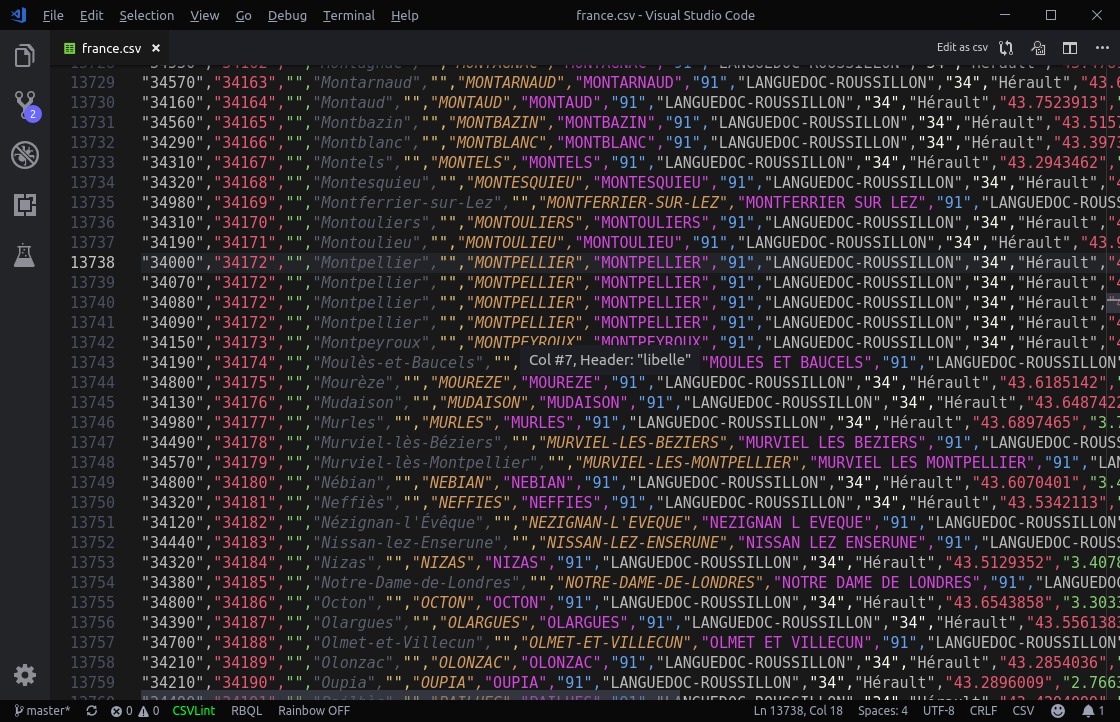
\includegraphics[width=0.85\textwidth]{img/csv.png}
	\caption{Fichier texte sous format CSV}
\end{figure}

\begin{figure}[!h]
	\centering
	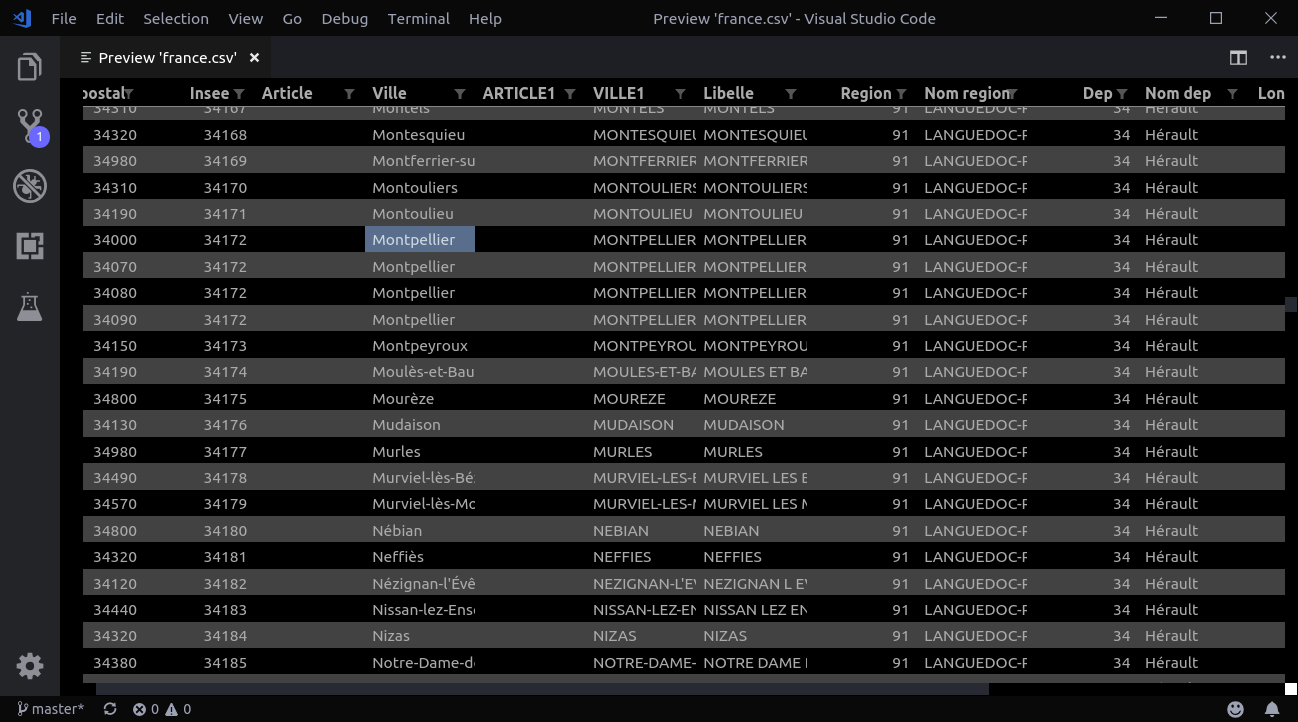
\includegraphics[width=0.85\textwidth]{img/csv_tables.png}
	\caption{Representation du même fichier en une table de données}
\end{figure}

Les champs texte peuvent également être délimités par des guillemets. Lorsqu'un champ contient lui-même des guillemets, ils sont doublés afin de ne pas être considérés comme début ou fin du champ. 
Si un champ contient un signe utilisé comme séparateur de colonne (virgule, point-virgule, tabulation, etc.), les guillemets sont obligatoires afin que ce signe ne soit pas confondu avec un séparateur.

\subsubsection{Lecture du fichier CSV}

Un fichier CSV est donc un moyen simple de stocker les données d'une base de données.
Ici on considére que :
\begin{itemize}
	\item Le nom du fichier (sans l'extensions) est le nom de la table.
	\item La première ligne du fichier ne represente pas des valeurs mais le nom des attributs de la table (c-à-d le nom des colones).
	\item Toutes les autres lignes represente des Tuples où chaque valeur est separée par une vergule.
\end{itemize}
\vspace{0.3cm}

La question qui se posent donc est :
\begin{center}
	\enquote{Comment lire et interprèter un fichier CSV ? et comment stocker les données qui en resulte ?}
\end{center}

\subsubsection{Lecture de la raquête SQL}

Maintenant qu'on a nos tables chargées en mémoire, il faut lire et interprèter la requête SQL\footnote{Structured Query Language: voir Page \pageref{sql}}.

Dans le contexe du projet, les requête prise en charge sont des requête SQL simples sans imbrication. Il respecteront donc la forme suivante : 

\enquote{SELECT nomAttribut1,nomAttribut2 FROM nomTable1,nomTable2 WHERE condition1 AND condition2 OR condition3}

Tel que : 
\begin{itemize}
	\item Le nom des attributs peuvent être remplacé par '*', ce qui signifie dans ce cas : \enquote{Tout les attributs};
	\item Il faut scpécifier au moin une table (dans le FROM);
	\item Les condition de selection (le WHERE) sont facultatif;
\end{itemize}
\vspace{0.3cm}


\subsection{Execution de la requête SQL}

La dernière étape consiste à executer la requête SQL, précédemment interprèter, sur les données charger en mémoire.
On peut clairement découper la requête SQL en 3 étapes :

\subsubsection{La projection}

La projection, ou sélection verticale, d'une table sur certaines de ses colonnes est une opération qui fournit une autre table ne contenant qu'un sous-ensemble des colonnes de la table initiale.

Soit la table "FRANCE" suivante :

\begin{tabular}{|l|c|r|}
	\hline
	ville   & region        & codepostal
	\\
	\hline
	Paris01 & Ile-de-france & 75101      \\
	Paris02 & Ile-de-france & 75102      \\
	Paris03 & Ile-de-france & 75103      \\
	\hline
\end{tabular}

La selection de la colonne ville et codepostal se fait par l'instruction :

\enquote{Select ville,codepostal from FRANCE;}

\begin{tabular}{|l|r|}
	\hline
	ville & codepostal
	\\
	\hline
	Paris01 & 75101  \\
	Paris02 & 75102 \\
	Paris03 & 75103 \\
	\hline
\end{tabular}

\subsubsection{La selection}

La sélection (sélection horizontale) permet de ne conserver que les tuples qui respectent une condition définie sur les valeurs des attributs, 
comme le but d'une requête SQL est d'extraire des informations spécifique dans des bases de données, 

La sélection permet :
\begin{itemize}
 	\item L'affichage de certaines lignes qui vérifient un critère donné;
	\item Le critère est une exrpession booléenne plus ou moins compliquée;
	\item Les conditions de sélection sont données juste après le mot clé WHERE;
	\item Les conditions sont séparer par des opérateur logique, AND et OR;
\end{itemize}
\pagebreak

Example de sélection :
soit la requête SQL suivante : 

\begin{center}
	\enquote{SELECT * FROM Employés WHERE age $\leq$ 30;}
\end{center}

Et la table : 
\begin{figure}[h]
	\begin{minipage}[c]{.46\linewidth}
		\centering
		\caption{Table 'Employés'}
		%\vspace{0.1cm}
		\begin{tabular}{|l|c|c|r|}
			\hline
			id   & nom  & age & idDep 
			\\
			\hline
			01 & Emp1 &  30  & 01 \\
			02 & Emp2 &  31  & 01 \\
			03 & Emp3 &  29  & 02 \\
			\hline
		\end{tabular}
	\end{minipage}
	\hfill%
	\begin{minipage}[c]{.46\linewidth}
		\centering
		\caption{Résultat de la sélection}
		\vspace{0.1cm}
		\begin{tabular}{|l|c|c|r|}
			\hline
			id   & nom   & age & idDep
			\\
			\hline
			01 & Emp1 &  30  & 01 \\
			03 & Emp3 &  29  & 02 \\
			\hline
		\end{tabular}
	\end{minipage}
\end{figure}

\subsubsection{La jointure}

la jointure est l'opération permettant d’associer plusieurs tables d'une base de données par le biais d’un lien logique de données entre les différentes tables, 
le lien étant vérifié par le biais d'un prédicat se situant dans la clause WHERE. Le résultat de l'opération est une nouvelle table. 
les tables données sont spécifier dans la partie FROM de la requête SQL.

La jointure entre une table A et B est une table composée de l'ensemble des couples possible entre leurs éléments respectant le prédicat.

Un exemple est plus parlant qu'une longue explication, prenons deux table Employés et Départements : 

\begin{figure}[h]
	\begin{minipage}[c]{.46\linewidth}
		\centering
		\caption{Table 'Employés'}
		\begin{tabular}{|l|c|c|r|}
			\hline
			id   & nom  & age & idDep 
			\\
			\hline
			01 & Emp1 &  30  & 01 \\
			02 & Emp2 &  31  & 01 \\
			03 & Emp3 &  29  & 02 \\
			\hline
		\end{tabular}
	\end{minipage}
	\hfill%
	\begin{minipage}[c]{.46\linewidth}
		\centering
		\caption{Table 'Départements'}
		\begin{tabular}{|l|c|c|r|}
			\hline
			idDep   & nom   & localisation
			\\
			\hline
			01 & Dep1 &  Montpellier  \\
			02 & Dep2 &  Paris  \\
			\hline
		\end{tabular}
	\end{minipage}
\end{figure}

	\enquote{SELECT * FROM Employés,Départements WHERE Employés.idDep = Départements.idDep}

\begin{figure}[h]
		\centering
		\caption{Execution de la jointure}
		\begin{tabular}{|l|c|c|c|c|r|}
			\hline
			id   & nom  & age & idDep & nom   & localisation 
			\\
			\hline
			01 & Emp1 &  30  & 01 & Dep1 &  Montpellier \\
			02 & Emp2 &  31  & 01 & Dep1 &  Montpellier \\
			03 & Emp3 &  29  & 02 & Dep2 &  Paris \\
			\hline
		\end{tabular}
\end{figure}


\subsection{Retourner le resultat}

La dernière étape consiste à renvoyer la table resultante de l'éxecution de la requête sous un format \textit{réutilisable} et \textit{compréhensible}.

\subsubsection{Réutilisable}

Il est question de stocker les données obtenu dans un fichier, sous un format CSV, pour qu'elles soit sauvgardées et réutilisablees par le programme.

\pagebreak

\subsubsection{Compréhensible}

Il s'agit de renvoyer la table de manière qu'elle soit compréhensible par l'utilisateur,c'est à dire en affichant les données sous forme d'un tableau.

\begin{figure}[h!]
		\centering
		\caption{Tableau}
		\vspace{0.1cm}
		\begin{tabular}{|l|c|r|}
			\hline
			id   & nom  & prenom 
			\\
			\hline
			01 & Nom1 &  Prenom1 \\
			02 & Nom2 &  Prenom2 \\
			03 & Nom3 &  Prenom3 \\
			\hline
		\end{tabular}
\end{figure}

\section{Objectif du programme}

L'objectif du programme est résume dans le schéma suivante :
\begin{figure}[!h]
	\centering
	% \includegraphics{} % Inserer ici le schéma ROLE DU PROGRAMME
	\vspace{0.1cm}
	\caption{Objectif du programme}
\end{figure}

% ------------------------------------- %
% Conception du Moteur de Requêtes
% ------------------------------------- %

\chapter{Conception du Moteur de Requêtes}

\section{Structure de données}
Avant toute chose, il faut commencer par charger les données en mémoire. Pour cela il faut commencer par savoir comment stocker efficacement les données pour pouvoir effectuer dessus les traitements demandés par l’utilisateur.

Pour cela nous avons donc réaliser un diagramme UML schématisant les classes utilisé pour stocker en mémoire l’ensemble des données utilisé pour la requête.

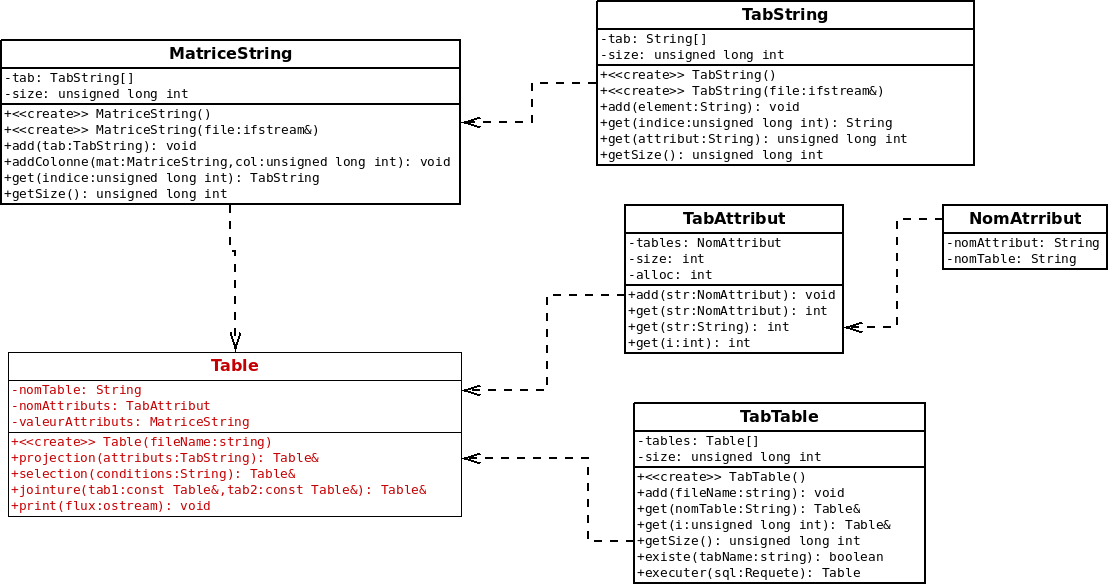
\includegraphics[width=1\textwidth]{img/sql.png}\par

La classe principale de notre programme est la classe « Table ». Comme vous le pouvez le voir sur le diagramme UML ci-dessus, la classe est constituée de trois attributs. Une chaîne de caractères dans laquelle on stock le nom de la table ( i.e : le nom du fichier ). Cette attribut est indispensable pour identifier la table sur laquelle on veux extraire les informations qu’on cherche.

On a aussi pensé a modélisé la classe TabString, ainsi que MatriceString et TabTable, pour simplifié l’utilisation des tableaux dynamiques. Ce qui a pour effet de produire du code facilement et cela rend donc sa lisibilité, son utilisation et sa maintenance beaucoup plus facile.

Le deuxième attribut de notre classe principale est un tableau de chaînes de caractères dans laquelle chaque case stockera le nom de la colonne concernée. Quant au troisième attribut, c’est une matrice à deux dimension qui se chargera de stocker les valeurs de notre table.

Notre programme commencera par initialiser un tableau de Table. Puis pour chaque fichier donné, il stockera la première ligne de ce dernier dans le deuxième attribut de la classe Table, puis continuera a lire le fichier pour stocker chaque ligne (i.e : à partir de la deuxième ligne) dans le troisième attributs.

Évidement, avant de stocker une ligne, nous la passons à une fonction qui se chargera de parser cette dernière séparent ainsi les différents attributs ( les attributs étant séparer par des virgule dans le fichier).

\section{Traitement des données}

Analyse de la requete => \enquote{select ... from ... where ...}

\subsection{La sélection}

\subsection{La projection}

Cette méthode, comme son nom l'indique, exécute une projection sut la Table Courante.

Le paramètre donnée est un TabString (tableau de chaîne de caractère) qui contient le nom des attributs à projeter.
On commence par déclarer une Table vide qui va contenir le résultat.
Le nom des attributs de cette table est initialiser à la de l'argument donné (l'objet TabString donné en paramètre).
Puis pour chaque élément d paramètre on ajoute la colonne correspondante à la table résultat.

\subsection{La jointure}
	\begin{figure}
		\centering
		\caption{Execution du produit cartésien}
		\begin{tabular}{|l|c|c|c|c|c|r|}
			\hline
			id   & nom  & age & Employés.idDep & Départements.idDep & nom   & localisation 
			\\
			\hline
			01 & Emp1 &  30 & 01 & 01 & Dep1 &  Montpellier \\
			02 & Emp2 &  31 & 01 & 01 & Dep1 &  Montpellier \\
			03 & Emp3 &  29 & 02 & 01 & Dep1 &  Montpellier \\
			01 & Emp1 &  30 & 01 & 02 & Dep2 &  Paris \\
			02 & Emp2 &  31 & 01 & 02 & Dep2 &  Paris \\
			03 & Emp3 &  29 & 02 & 02 & Dep2 &  Paris \\
			\hline
		\end{tabular}
	\end{figure}
% ------------------------------------- %
% Implementation
% ------------------------------------- %

\chapter{Implementation}

\section{Choix de la téchnologie}

\section{Développement}

fonctions en plus / implem des algo avec appel aux differentes fonctions des objets….

\subsection{Chargement des données}

\subsection{restitution des données (affichage)}

\subsection{Selection ...}

\section{Logiciel}

terminal / ligne de commande / formt des données en entrée et sortie

\section{Test}


% ------------------------------------- %
% Bilan et difficultés rencontrées
% ------------------------------------- %

\chapter{Bilan et difficultés rencontrées}

% ------------------------------------- %
% Perspective
% ------------------------------------- %

\chapter{Perspective}

% ------------------------------------- %
% Annexes
% ------------------------------------- %

\chapter{Annexes}


\end{document}
